\documentclass[tikz, border=0px]{standalone}
\usepackage{tikz}
\usetikzlibrary{shapes,arrows}

\tikzstyle{startstop} = [rectangle,rounded corners,minimum width=3cm,minimum height=1cm,align=center,draw=black, text width=2.5cm, fill=green!30]

\tikzstyle{therapy} = [trapezium, trapezium left angle =70, trapezium right angle=110, minimum width=2cm, minimum height = 1cm, centered,draw=black,align=center, text width=2cm, fill=orange!30]

\tikzstyle{decision} = [diamond, minimum width = 3cm, minimum height = 3cm, text centered, draw=black, text width = 2cm,align=center,fill=blue!30]

\tikzstyle{arrow} = [thick, ->, >=stealth]
\tikzstyle{doublearrow} = [<->, thick, >=stealth]

\begin{document}
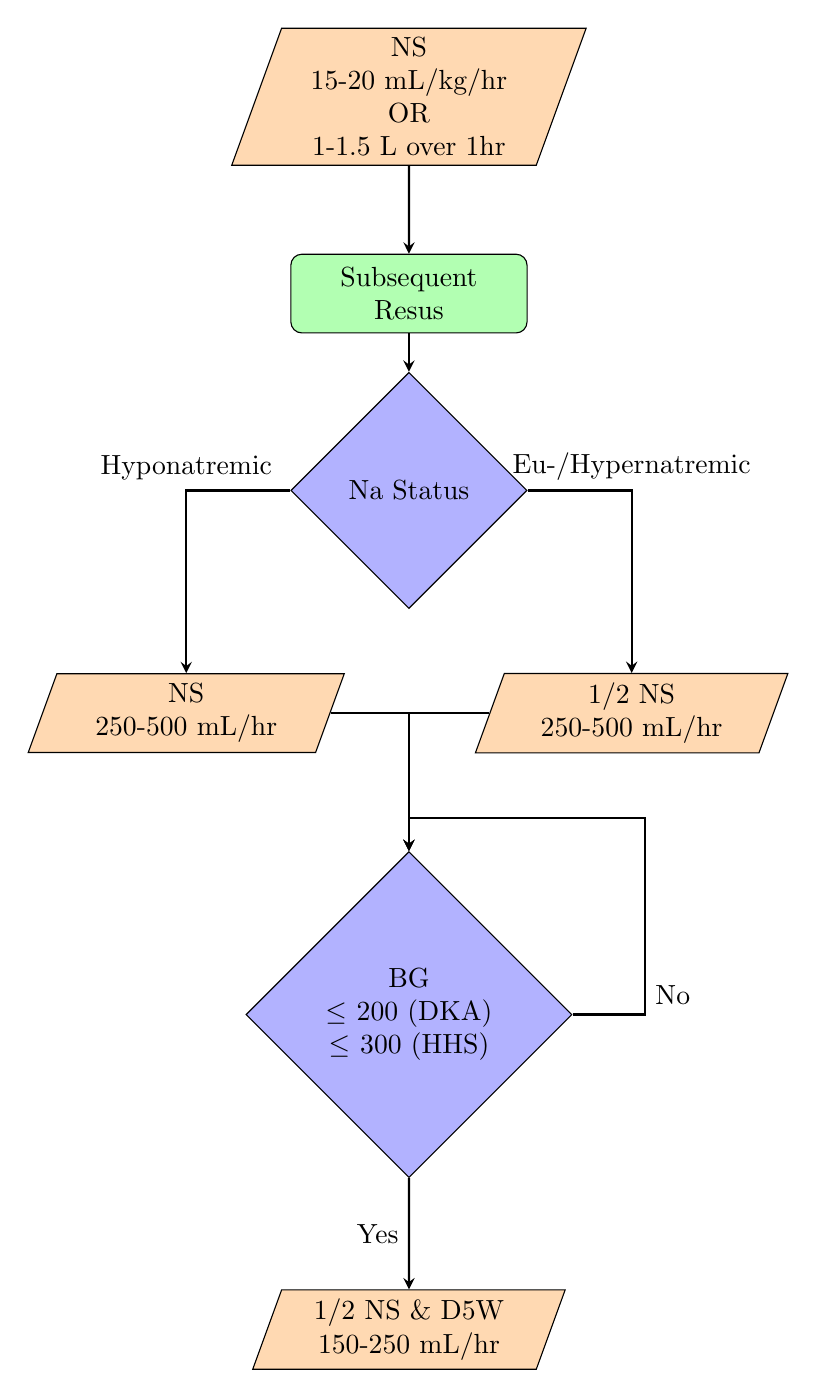
\begin{tikzpicture}[node distance=4cm]

\node(start) [therapy, text width=3cm] {NS\\ 15-20 mL/kg/hr\\ OR\\ 1-1.5 L over 1hr};

\node(subsequent) [startstop, below of=start, yshift=1.5cm] {Subsequent Resus};

\node (sodiumStatus) [decision, below of=subsequent, yshift=1.5cm] {Na Status};

\node (hyponatremic) [therapy,below left of=sodiumStatus, text width=3cm] {NS\\ 250-500 mL/hr};
\node (hypernatremic) [therapy,below right of=sodiumStatus, text width=3cm] {1/2 NS\\ 250-500 mL/hr};

\node (glucoseStatus) [decision, below left of=hypernatremic, text width=2.5cm, yshift=-1cm] {BG\\ $\le 200$ (DKA)\\ $\le 300$ (HHS)};

\node (normoglycemic) [therapy, below of=glucoseStatus,text width=3cm] {1/2 NS \& D5W\\ 150-250 mL/hr};

\draw [arrow] (start) -- (subsequent); 
\draw [arrow] (subsequent) -- (sodiumStatus);

\draw [arrow] (sodiumStatus) -| node [anchor = south] {Hyponatremic} (hyponatremic);
\draw [arrow] (sodiumStatus) -| node [anchor = south] {Eu-/Hypernatremic} (hypernatremic);
\draw [arrow] (hyponatremic) -| (glucoseStatus);
\draw [arrow] (hypernatremic) -| (glucoseStatus);
\draw [arrow] (glucoseStatus) -- node [anchor = east] {Yes} (normoglycemic);
\draw [arrow] (glucoseStatus) -- ++(3cm,0) node [anchor = south west] {No} -- ++(0,2.5cm) -| (glucoseStatus);


\end{tikzpicture}
\end{document}